A 5G network hash RAN with user equipments and 
\begin{figure}[htbp]
	\centering
       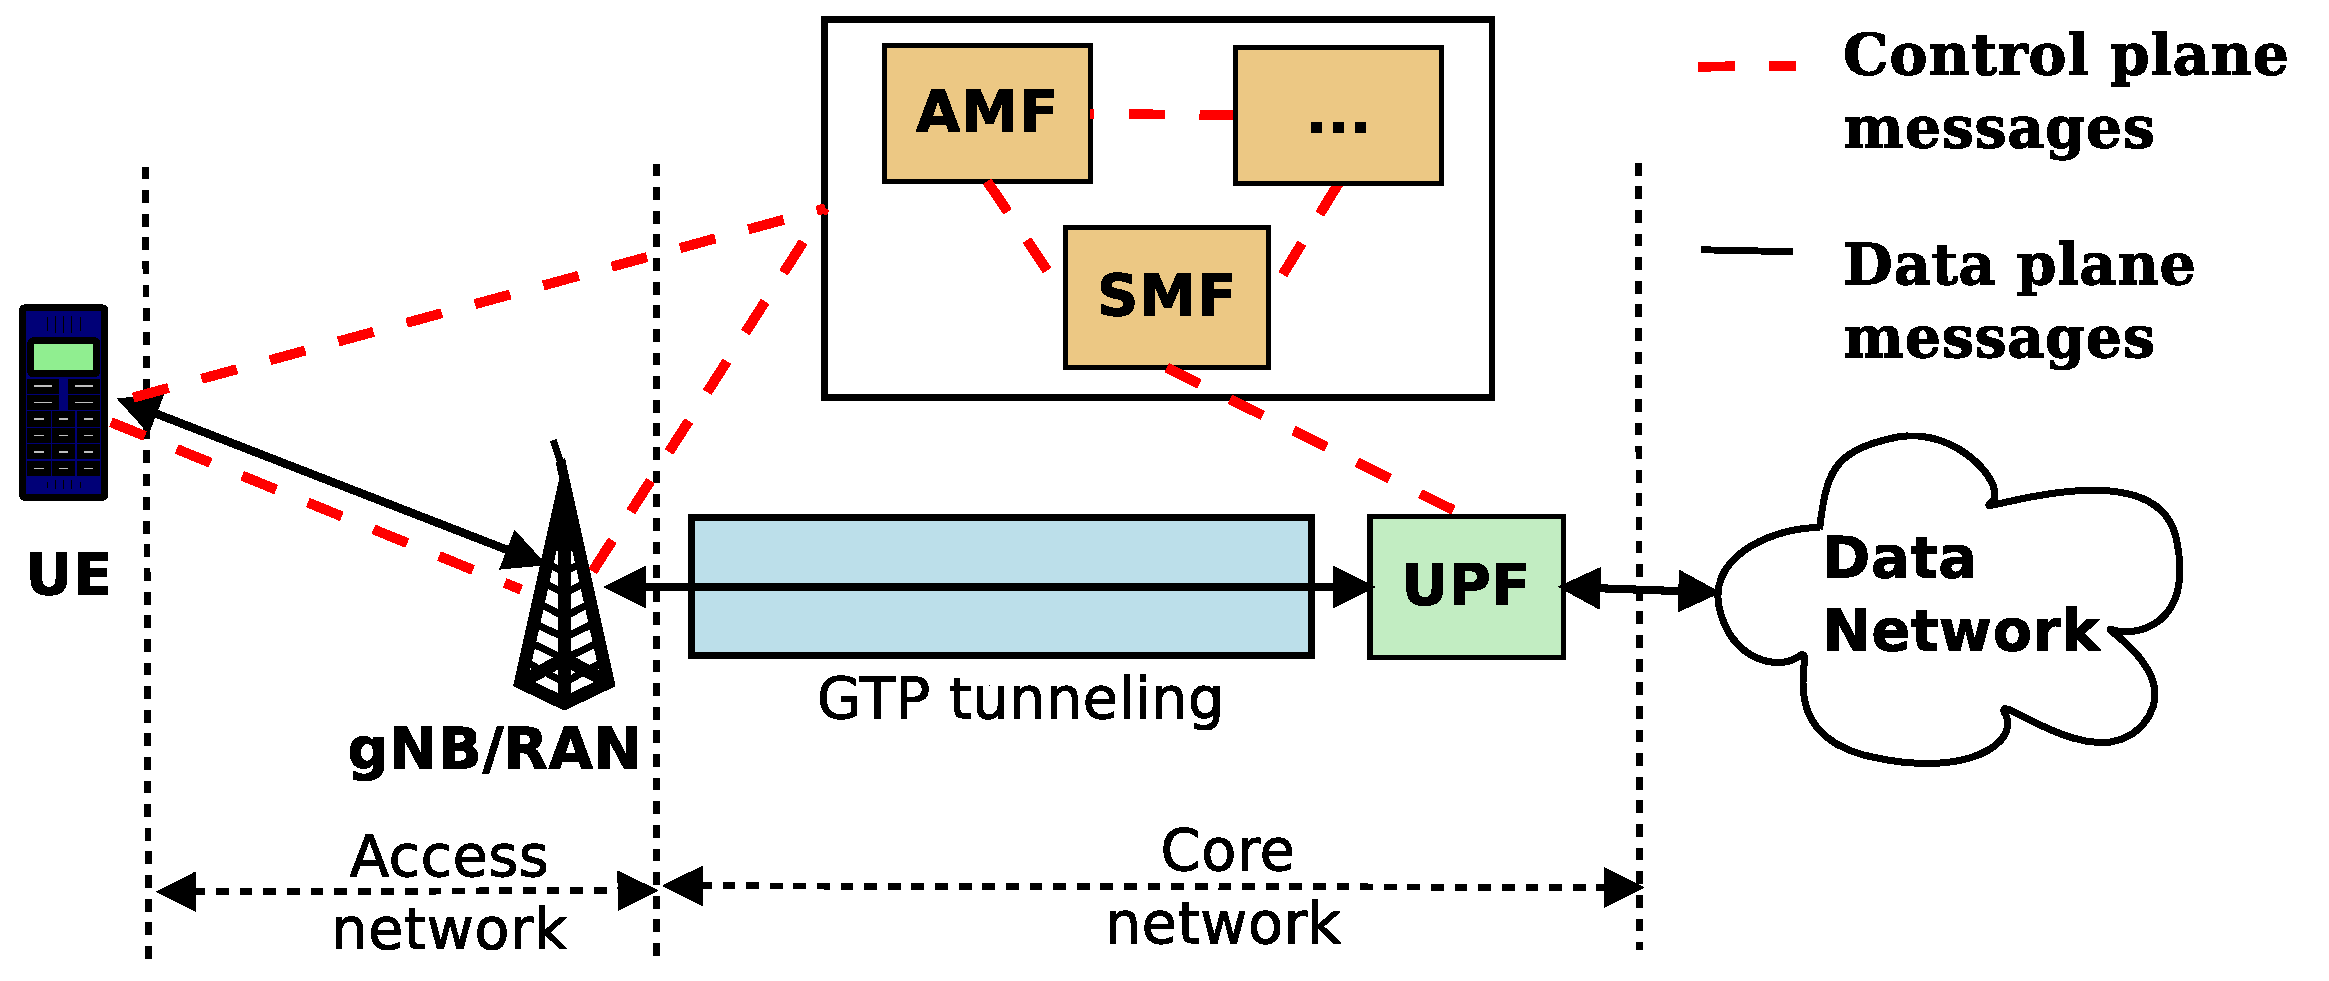
\includegraphics[width=0.7\textwidth]{fig/5g_arch.eps}
       %  \setlength{\abovecaptionskip}{-2pt}
       \setlength{\belowcaptionskip}{-12pt}
	\caption{5G Architecture.}
	\label{fig:5g_arch}
       \end{figure}
       %\vspace{-5mm}
       




\section {PFCP Protocol\label{sec:PFCP}}
 \begin{figure}[htbp]
    \centering
    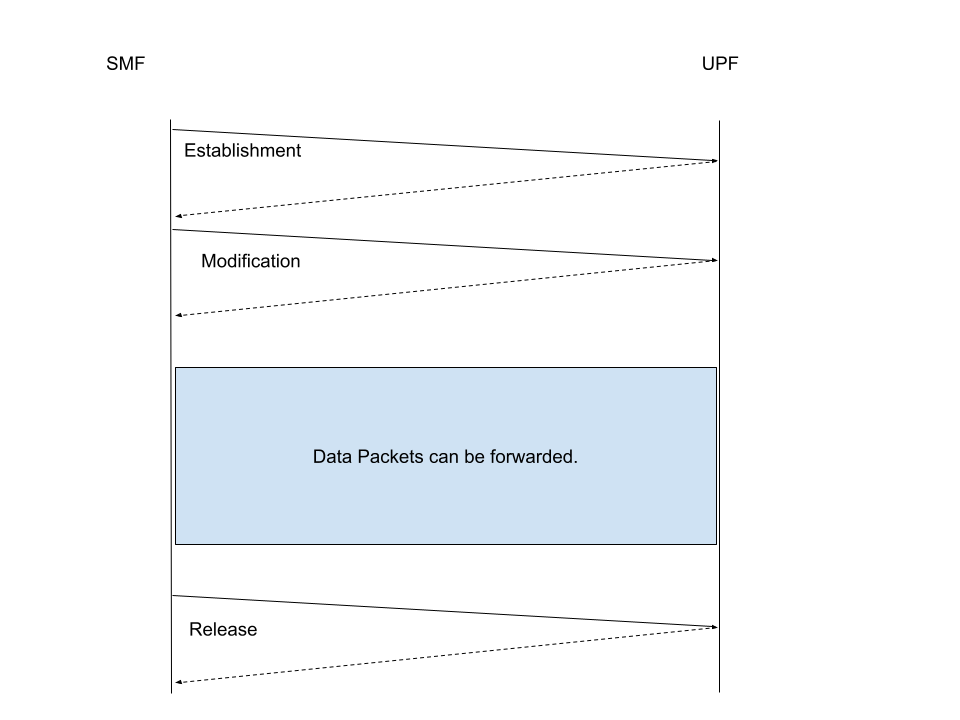
\includegraphics[width=0.7\textwidth, keepaspectratio]{./fig/Introduction/PFCP.png}
    \caption{PFCP Session Messages}
    \label{fig:PFCP}
\end{figure}

PFCP stands for Packet Forwarding Control Protocol. 
 There are two types of messages sent using PFCP - node related and session related.
 The discussion here describes session related messages.

 Session Management Function (SMF) interacts with the User Plane Function (UPF) to setup sessions related 
 information at the UPF.
This  information enables UPF to identify data packets of different sessions coming from RAN 
and provide forwarding, usage report, charging, buffering, QoS related service to the sessions.
Each session is identified by a unique session ID which helps in differentiating 
among different UEs/sessions at the UPF. 

There are three kinds of messages sent from SMF to the UPF in PFCP session related messages-
\begin{itemize}
	\item \textbf{Establishment Request} This message has all the forwarding, usage report, QoS etc. related information for  a new UE session.  
	\item \textbf{Modification Request} Once the establishment response is
	received from the UPF, the UPF sends the modification request. The important field in this message is the intimation of identifier that will be used for data plane packets coming from the UPF. The data forwarding can not start before the modification response is received.
	\item \textbf{Release Request} Once the session is not required, th release 
	request is sent to the UPF signaling the tear down of the session and UPF
	 may remove this session's related information.
\end{itemize}
UPF gives response to each of the three messages. 
\section {GTP Protocol\label{secGTP}}
The raw packets meant for communicating outside the netowrk are encapsulated with GTP  application level 
header. GTP runs over UDP/IP stack. This GTP header  (shown in \ref{figGTPheader})contains various fields for regulating the
 session parameters. The relevant fields are
 \begin{figure}[htbp]
    \centering
    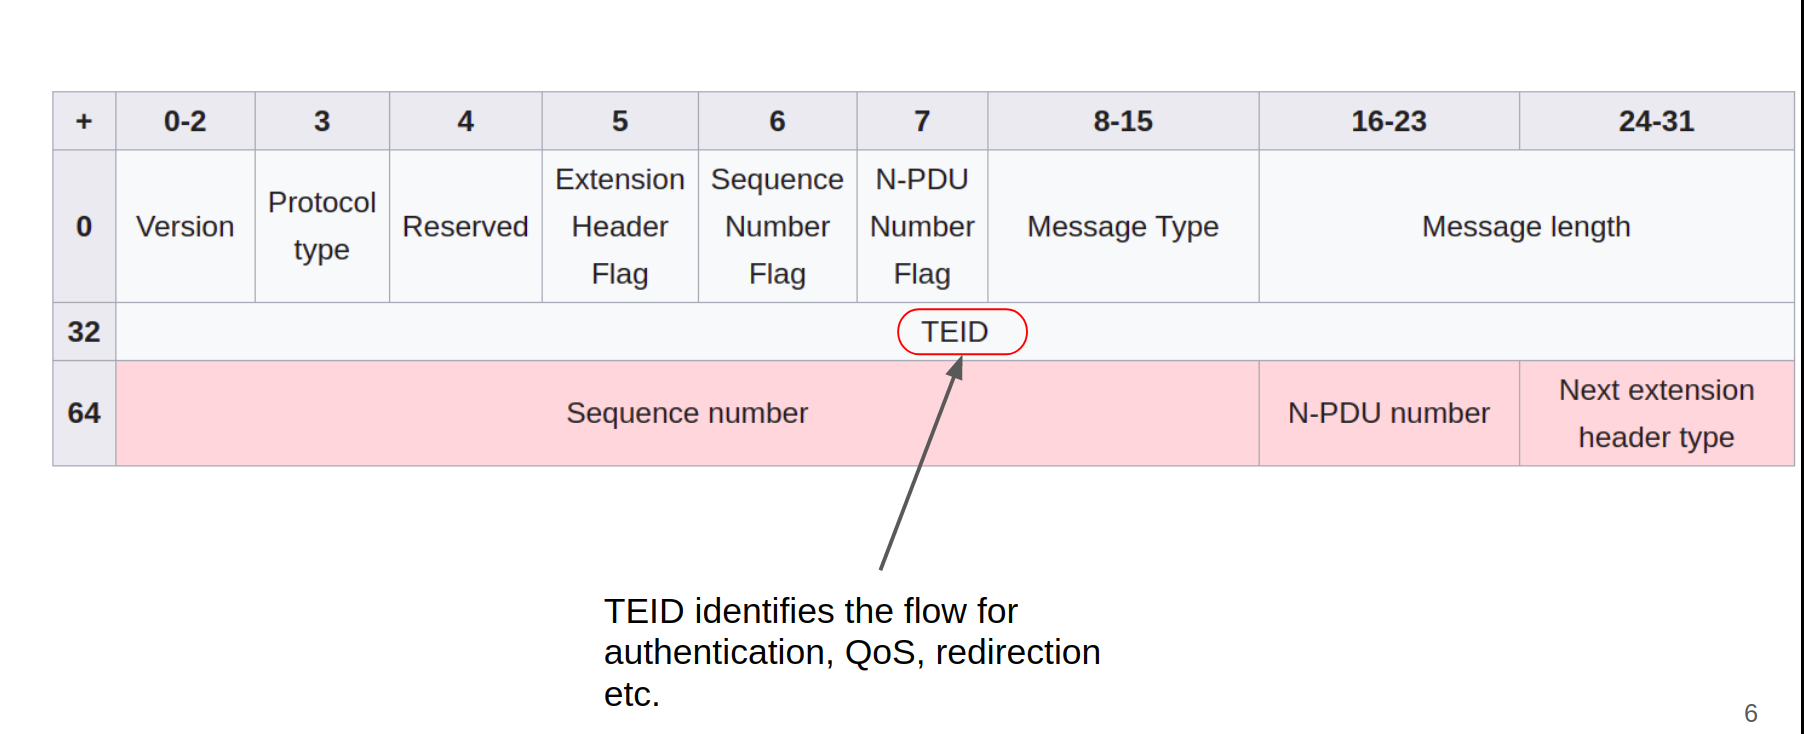
\includegraphics[width=0.7\textwidth, keepaspectratio]{./fig/Introduction/intro2.png}
    \caption{GTP-U header \cite{gtpwiki}}
    \label{figGTPheader}
\end{figure}
 \begin{itemize}
    \item \textbf{Tunnel Endpoint Identifier (TEID)} identifies the packet with a particular session which may have different Quality of Service parameters.
    \item \textbf{Extension Headers} These are required for providing differentiated services to  a given packet in the same or different session.
 \end{itemize}

